<<<<<<< HEAD
\documentclass[12pt]{article}

\usepackage[a4paper, margin=1in]{geometry} % Margins
\usepackage{fancyhdr} % Set header and footer
\usepackage{titling}

\usepackage[T1]{fontenc} % For international characters
\usepackage{XCharter} % XCharter as the main font

\usepackage[
  backend=biber,
  style=numeric,
  citestyle=authoryear,
  sorting=none
  ]{biblatex}
\addbibresource{./Ref/reference.bib}

\usepackage[english]{babel} % Use english by default
\usepackage{csquotes}

\usepackage{amsmath, amsthm, amssymb, amsfonts, mathtools}
\usepackage{graphicx}
\usepackage{tikz}
\usetikzlibrary{shapes, arrows}
% \usepackage[]{algorithm2e}
% \usepackage{caption, enumerate}
% \usetikzlibrary{graphdrawing, shapes}
% \usegdlibrary{trees}

\usepackage{hyperref}
\hypersetup{
  colorlinks,
  citecolor=black,
  filecolor=black,
  linkcolor=black,
  urlcolor=black
}

\pagestyle{fancy}
\fancyhf{}
\fancyhead[R]{Leo W.}
\fancyfoot[R]{\thepage}
\setlength{\headheight}{15pt}

%----------------------------------------------------------------------------------------
%	CUSTOM COMMANDS
%----------------------------------------------------------------------------------------

\newcommand{\articletitle}[1]{\renewcommand{\articletitle}{#1}} % Define a command for storing the article title
\newcommand{\articlecitation}[1]{\renewcommand{\articlecitation}{#1}} % Define a command for storing the article citation
\newcommand{\doctitle}{\articlecitation\ --- ``\articletitle''} % Define a command to store the article information as it will appear in the title and header
\newcommand{\doctitlenocite}{\articletitle} % No citation

\newcommand{\datenotesstarted}[1]{\renewcommand{\datenotesstarted}{#1}} % Define a command to store the date when notes were first made
\newcommand{\docdate}[1]{\renewcommand{\docdate}{#1}} % Define a command to store the date line in the title

\newcommand{\docauthor}[1]{\renewcommand{\docauthor}{#1}} % Define a command for storing the article notes author

\newcommand{\bookcitation}[1]{\renewcommand{\bookcitation}{#1}} % Define a command for storing the book citation

% Define a command for the structure of the document title
\newcommand{\printtitle}{
\begin{center}
\textbf{\Large{\doctitle}}

\docdate

\docauthor
\end{center}
}

% No citation
\newcommand{\printtitlenocite}{
\begin{center}
\textbf{\Large{\doctitlenocite}}

\docauthor

\docdate
\end{center}
}

%----------------------------------------------------------------------------------------
%	STRUCTURE MODIFICATIONS
%----------------------------------------------------------------------------------------

\setlength{\parskip}{3pt} % Slightly increase spacing between paragraphs

% Uncomment to center section titles
% \usepackage{sectsty}
% \sectionfont{\centering}

% Uncomment for Roman numerals for section numbers
% \renewcommand\thesection{\Roman{section}}
% \renewcommand\thesubsection{\thesection.\Roman{subsection}}


\title{Momentum Strategy Enhancement \\ with Machine Learning \\[2ex]
  \large Sector-based Random Forest Application \\[4ex]
  \large COMP4971C - Independent Work (Fall 2019)}
\author{WONG Jia Yeung, Leo}
\date{November, 2019}

\begin{document}

\begin{titlingpage}
  \maketitle
  \begin{abstract}
    In this research project, the feasibility of improving "plain" momentum strategy with machine learning method (Random Forest) in financial portfolio construction and optimisation is examined, while simultaneously testing the market efficiency of the Hong Kong stock market.
  \end{abstract}
\end{titlingpage}

\fancyhead[L]{Multi-Factor Portfolio Optimisation with Machine Learning}

\tableofcontents


\section{Introduction}

The finance industry is one of the major driving forces of Hong Kong. Portfolio construction and optimisation has always been a tedious work for discretionary asset managers and individual investors. With the increasing integration and popularity of machine learning techniques in various industries, the finance industry provides an experimental field with great incentives.

To narrow down the scope of research, a simple long-short momentum strategy is used to constrct a stock-only portfolio, focusing on the Hong Kong stock market. This project examines the prediction power of random forest model and compare the findings against benchmark (without any machine learning enhancement).


\section{Disclaimer}

The information presented in this research is not intended as, and shall not be understood as financial advice to enter in any security transactions or to engage in any of the investment strategies.


\section{Data, Tools and Evaluation}

\subsection{Data}

We use data of listed Hong Kong companies from Refinitiv by Blackstone Group and Thomson Reuters.

We obtain all companies that are currently (July 2019) listed or have been listed on the HKEX from Refinitiv from January 2000 to June 2019 to eliminate survivorship bias. We then obtain corresponding daily price/volume data and recompile the index to align different companies.

We report the distribution of companies (raw data) in Figure \ref{fig:sector_dist}, split by TRBC\footnote {Thomson Reuters Business Classification System} economic sector.

\begin{figure}[h]
  \begin{center}
    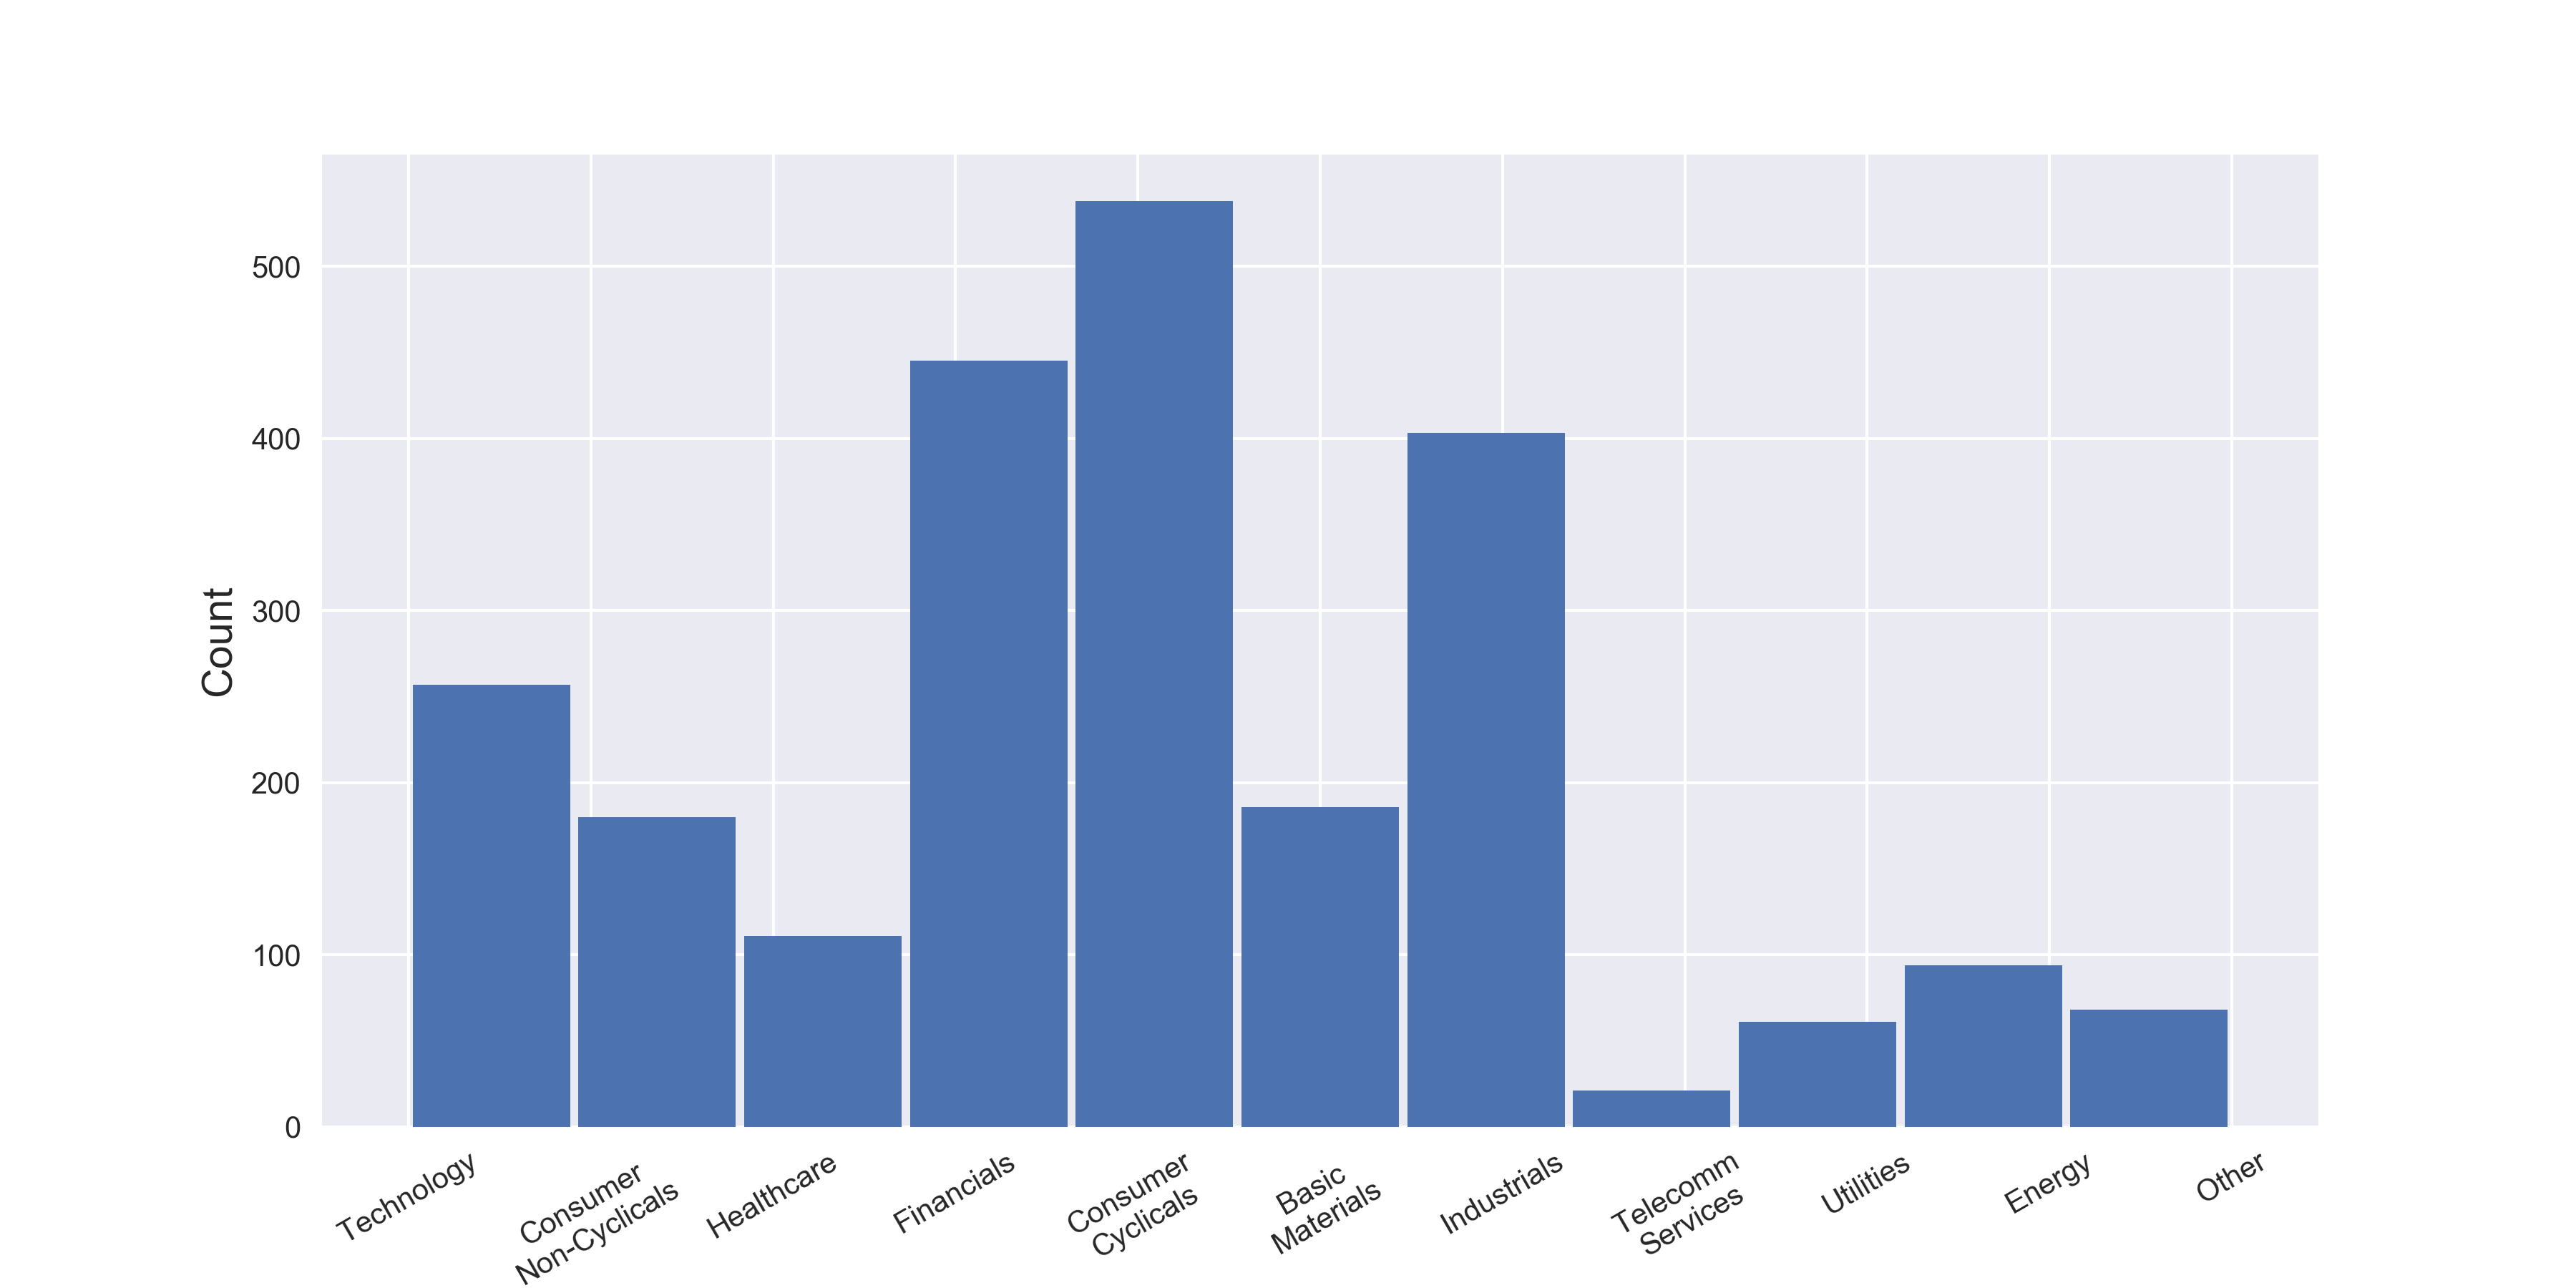
\includegraphics[width=1\linewidth]{figure/sector_dist.png}
  \end{center}
  \caption{Distribution of TRBC Economic Sector}
  \label{fig:sector_dist}
\end{figure}

\subsection{Tools}

Backtest and data processing is conducted in Python 3.7 with Jupyter kernels using numpy and pandas. We use sci-kit learn for the Random Forest model, trained on CPUs.

\subsection{Evaluation Metrics}

Sharpe ratio and win rate are the two main evaluation metrics.

\subsubsection{Sharpe Ratio}

Sharpe ratio was first introduced by \cite{sharpe1966}. It measures the expected return gained per unit of risk taken for a zero investment strategy. According to the definition in \cite{sharpe1994}, assume \(R_{Pt}\) as a \(t\)-period return series, \(R_{ft}\) as the risk-free rate series over the same period. Then the Sharpe ratio \(S_h\) from \(t=1\) to \(t=T\):

\begin{align*}
  S_h &\equiv \frac{\overline{D}}{\sigma_D} \\
  \text{where}~D &\equiv R_{Pt} - R_{ft} \\
  \overline{D} &\equiv \frac{1}{T} \sum_{t=1}^T D_t \\
  \sigma_D &\equiv \sqrt{\frac{\sum_{t=1}^T (D_t-\overline{D})^2}{T-1}}
\end{align*}

\subsubsection{Win Rate}

Win rate is expressed as the ratio of profiting time to the total investment timespan. Let \(\pi_t\) be the profit/loss of a strategy at time \(t\), \(T\) be the total number of steps (timespan). Assume the profit/loss is non-zero at every time \(t\), i.e. \(n_{\pi=0} = 0\), then \(T = n_{\pi<0} + n_{\pi>0}\). Let \(w\) be the win rate, \(pf\) be the profit factor, \(pr\) be the payoff ratio, \(RoR\) be the risk of ruin.

\begin{align*}
  w &\equiv \frac{n_{\pi>0}}{n_{\pi<0} + n_{\pi>0}} \\
\end{align*}


\section{Methodology}

Our methodology consists of four stages. First, we split the data into training and test sets. Second, we discuss the feature space for training and prediction. Third, we describe the random forest model. Fourth, we apply the trading strategy.

\subsection{Training/Test Sets Split}

We define multiple non-overlapping train-test combination sets to avoid information leak. A train-test combination consists of a training period lasting 750 transaction days (approximately 3 years) and a test period of 250 days (approximately 1 year, \cite{Fischer2017Deep}). We split the dataset from 2000 to 2015 into 4 non-overlapping study periods.

\subsection{Feature Generation/Selection}

We currently use "momentum" based features, i.e., we adopt a "lookback" period which $l$-timesteps of historical price data is reviewed and used for feature computation. We take a simple return of security $s$ during the time interval from $t-l$ to $t$ as the input.

$$r_{t-l, t}^s = \frac{P_t^s}{P_{t-l}^s}-1$$

Note that the input feature (return) is normalised accross the sector $m$, i.e.,

$$\tilde{r}_{t-l, t}^s = \frac{r_{t-l, t}^s-\mu_{t-l, t}^m}{\sigma_{t-l, t}^m}$$

We define a 3-class classification problem, the dependent variable $y_{t, t+h}^s|t$ can have 3 different values. We adopt a "holding" period that we review data upto timestep $t+h$ and compute the returns $r_{t, t+h}^s$ and sort the results. Class $1$ refers to the securities in the upper third of the ranking. Class $-1$ and $0$ refer to the securities in the lower and middle third respectively. We design the definition to maintain balanced classes.

\subsection{Random Forest Model}

We use random forest as an overlay of the original momentum signal. The model aims to improve the quality of the raw signals by unvealing hidden patterns accross different securities over the same time period. We set the number of estimators to $100$ and use default configuration for other parameters.

\subsection{Trading Strategy}

We adopt a simple long-short strategy.

First, classify each stock $s_i \in S$ at $t+h$ given the information upto $t$. Second, compute the prediction confidence to obtain a weight matrix for trade execution. Third, long the top $k\%$ and short the bottom $k\%$ to create a long-short portfolio consisting of $2k\%$ stocks as the top securities are the most undervalued and the bottom ones are the most overvalued, currently $k = 5$.

The same procedures are performed on both the random forest model and raw signals.


\section{Result*}

The random forest model shows significant Sharpe ratio and win rate improvement in most most cases regardless of the sector and test periods.

\begin{figure}[h]
  \begin{center}
    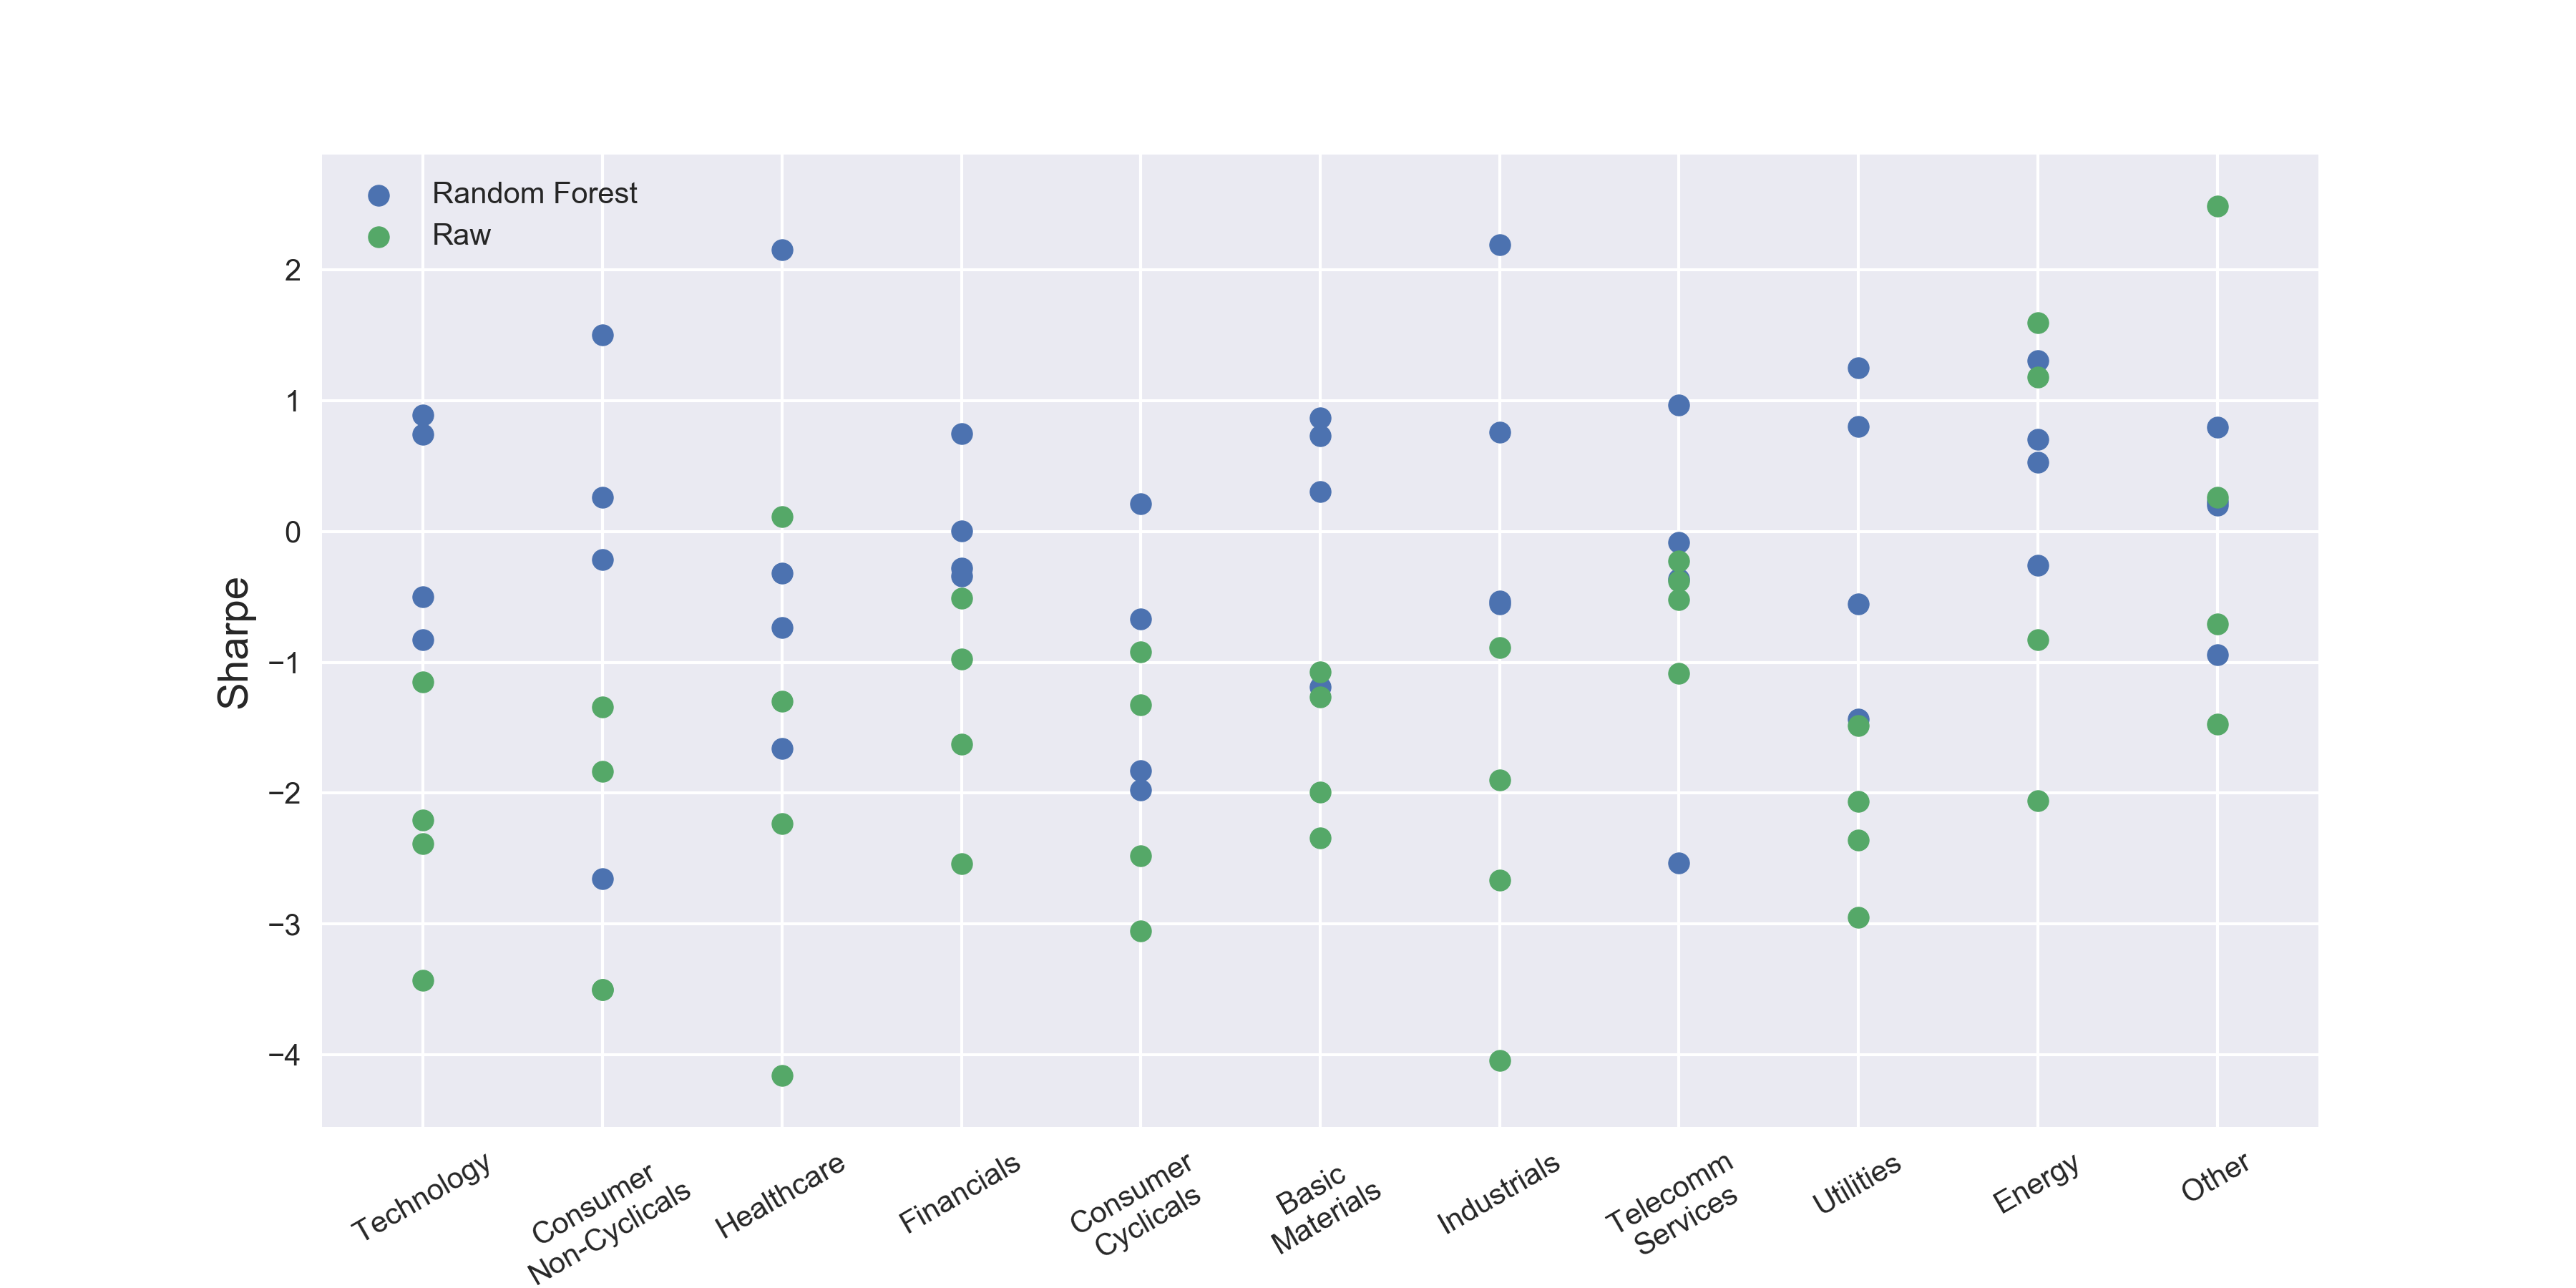
\includegraphics[width=1\linewidth]{figure/rf_raw_sharpe.png}
  \end{center}
  \caption{Sharpe Comparison of RF Model and Raw}
  \label{fig:rf_raw_sharpe}
\end{figure}

\begin{figure}[h]
  \begin{center}
    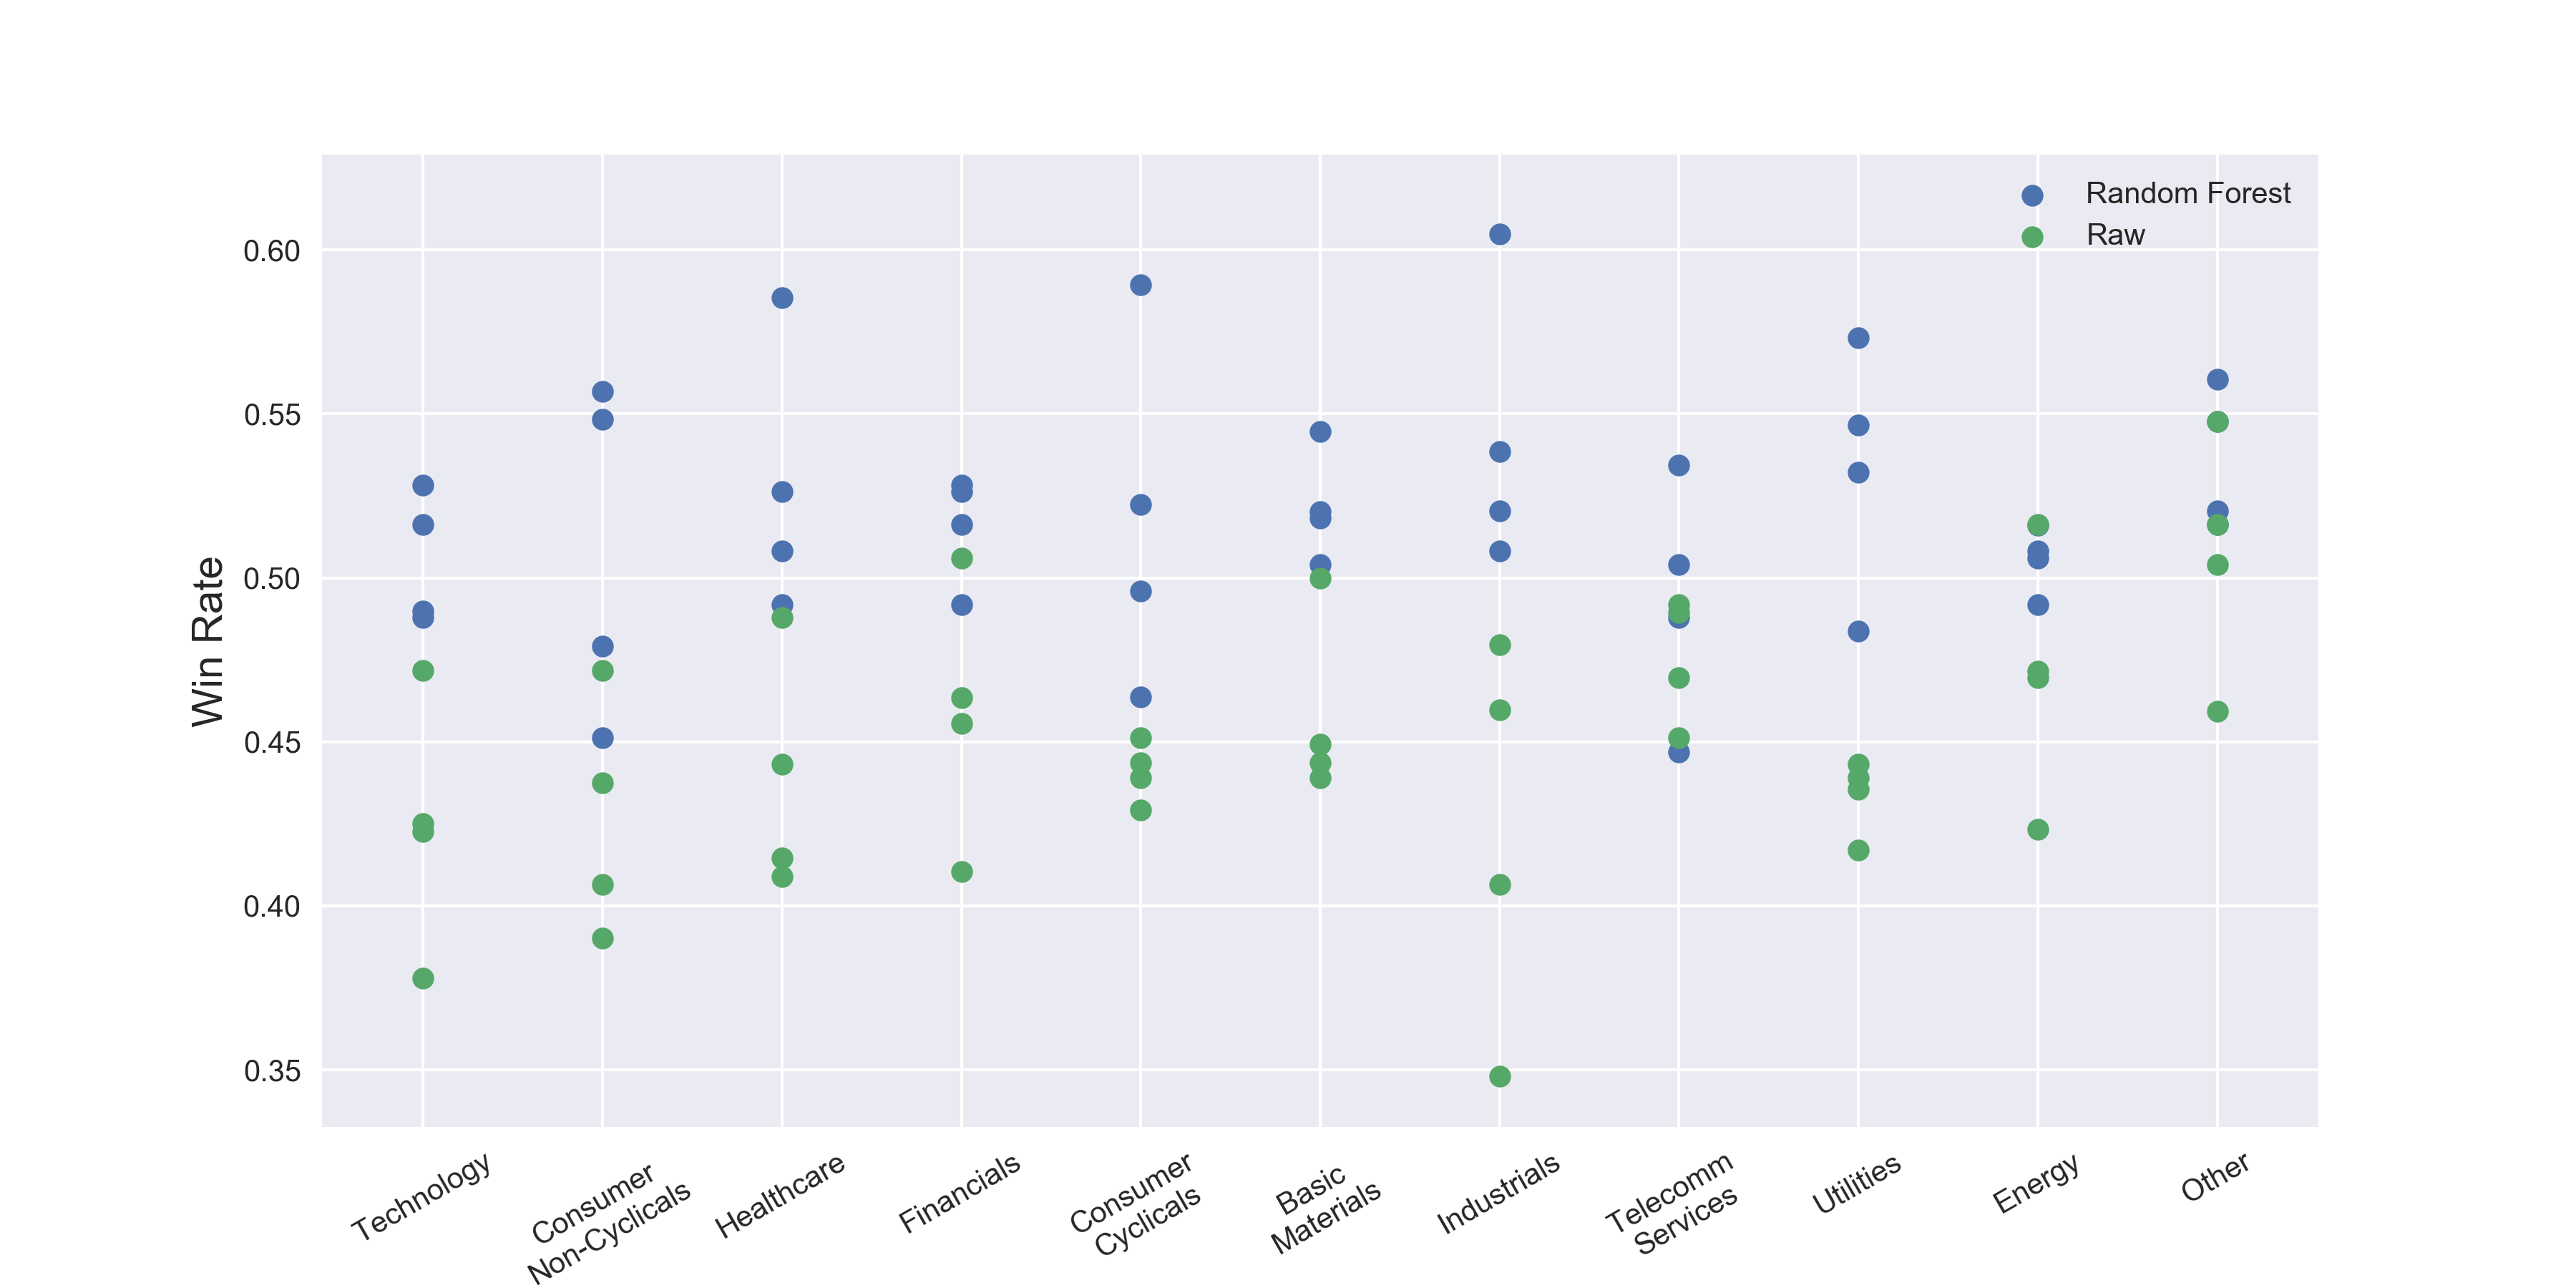
\includegraphics[width=1\linewidth]{figure/rf_raw_win_rate.png}
  \end{center}
  \caption{Win Rate Comparison of RF Model and Raw}
  \label{fig:rf_raw_win_rate}
\end{figure}

\section{Conclusion*}


\section{Future Work}

We may expand our work to overcome current constraints, including but not limited to data problem, resource limitation.

Due to data limitations, we are restricted to only price/volume data at a daily frequency. The lack of variaty and relatively low frequency hinder the testing of more complex asset pricing models, trading strategies, as well as complex machine learning methods.


\section{Appendix*}


\renewcommand{\refname}{Reference} % Change the default bibliography title
\printbibliography

\end{document}
